\documentclass[10pt,twoside,openright]{memoir}

% MATH
\usepackage{amsmath,amsthm,amssymb,scalerel}
\usepackage{bm}
\usepackage{mathtools,thmtools}
\usepackage{tcolorbox}

% GRAPHICS
\usepackage{import}

\usepackage{graphicx}
\usepackage{tikz}
\usepackage{pgfplots}
\usepackage{rotating}
\usetikzlibrary{
  matrix,
  external,
  arrows.meta
}
\tikzexternalize[prefix=pdf/]
% \tikzset{external/system call={pdflatex \tikzexternalcheckshellescape -halt-on-error
%   -interaction=batchmode -jobname "\image" "\texsource" && % or ;
%   pdftops -f 1 -l 1 -eps "\image".pdf}}
\tikzset{external/system call={pdflatex \tikzexternalcheckshellescape -halt-on-error
  -interaction=batchmode -jobname "\image" "\texsource" && % or ;
  pdfseparate -f 1 -l 1 "\image".pdf "\image"_tmp.pdf &&
  mv "\image"_tmp.pdf "\image".pdf}}


% LAYOUT
\usepackage{lipsum}  
\usepackage[utf8]{inputenc}
\usepackage[T1]{fontenc}
\usepackage[english]{babel}
\usepackage{subcaption}
\usepackage{fmtcount}
\captionsetup{font+=smaller,labelfont={sc,bf},labelsep=period}
\captionsetup[sub]{labelformat=simple,labelsep=period}
\def\onefigwidth{\textwidth}
\def\twofigwidth{0.475\textwidth}
\def\threefigwidth{0.3\textwidth}

\chapterstyle{dash}
\renewcommand*{\thechapter}{\arabic{chapter}}
\renewcommand*{\printchaptername}{---\enspace\normalfont\slshape{\Ordinalstring{chapter}[f] chapter}\enspace---\centering}
\renewcommand\chaptitlefont{\normalfont\huge\scshape\bfseries\centering}
\renewcommand\printchapternum{}

% Remove centred footer pagenumber on first page of part and chapter
\copypagestyle{chapter}{plain}% Copy plain page syle to chapter page style
\makeoddfoot{chapter}% Adjust odd footer for chapter page style
  {}% Left odd footer
  {}% Center odd footer
  {}% Right odd footer

\copypagestyle{part}{plain}% Copy plain page syle to part page style
\makeoddfoot{part}% Adjust odd footer for part page style
  {}% Left odd footer
  {}% Center odd footer
  {}% Right odd footer

% TABLE OF CONTENTS STYLE
\setsecnumdepth{subsection}
\renewcommand*{\cftpartfont}{\normalfont\LARGE\scshape\bfseries}
\renewcommand*{\cftchapterfont}{\normalfont\scshape\bfseries}
\renewcommand*{\cftsectionfont}{\normalfont}
\renewcommand*{\cftsubsectionfont}{\normalfont}

\usepackage{titletoc}
\usepackage{libertine}
\setcounter{tocdepth}{2}

\makeatletter
\renewcommand{\partnumberline}[1]{{\normalfont\normalsize\slshape ---\enspace Part #1\enspace ---}\\}
\renewcommand*{\l@part}[2]{%
  \ifnum \c@tocdepth >-2\relax
    \cftpartbreak
    \begingroup
      {
        \setlength{\memRTLleftskip}{0pt}
        \setlength{\memRTLrightskip}{0pt}
        \interlinepenalty\@M
        \centering
        \cftpartfont #1
        \par
      }
      \nobreak
        \global\@nobreaktrue
        \everypar{\global\@nobreakfalse\everypar{}}%
    \endgroup
    \cftpartbreak
  \fi}
\makeatother



% PART STYLE
\renewcommand*{\thepart}{\arabic{part}}
\renewcommand*{\parttitlefont}{\normalfont\Huge\bfseries\scshape}
\renewcommand*{\partnamefont}{\normalfont\slshape}
% \renewcommand*{\partnumfont}{\normalfont\scshape\MakeLowercase}
\renewcommand*{\printpartname}{---\enspace\partnamefont{\Ordinalstring{part}[f] part}\enspace---}
% \renewcommand*{\printpartname}{\decofourleft\enspace\partnamefont{\Ordinalstring{part}[f] part}\enspace\decofourright}
\renewcommand*{\printpartnum}{}

\setsecheadstyle{\centering\large\bfseries\scshape}
\setbeforesecskip{-1\onelineskip plus -1ex minus -.2ex}
\setaftersecskip{1\onelineskip plus .2ex}

\setsubsecheadstyle{\centering\scshape} 
\setbeforesubsecskip{-1\onelineskip plus -1ex minus -.2ex}
\setaftersubsecskip{1\onelineskip plus .2ex}

\setsubsubsecheadstyle{\centering\scshape} 
\setbeforesubsubsecskip{-1\onelineskip plus -1ex minus -.2ex}
% \setaftersubsubsecskip{1\onelineskip plus .2ex}

% HEADERS AND FOOTERS
\makeatletter
\renewcommand{\chaptermark}[1]{%
  \markboth{%
    \ifnum\c@secnumdepth>\m@ne
      \@chapapp\ {\footnotesize\thechapter}. \ %
    \fi
  #1%
  }{}%
}
\renewcommand{\sectionmark}[1]{%
  \markright{%
  \ifnum \c@secnumdepth >\z@
    {\footnotesize\thesection}. \ %
  \fi
  #1%
  }{}%
}
\makeatother

\makeevenhead{headings}{\thepage}{}{\normalfont\small\scshape\leftmark}
\makeoddhead{headings}{\normalfont\small\scshape\rightmark}{}{\thepage}

%% ABSTRACT PER CHAPTER
\AtBeginDocument{
  \renewcommand{\abstractname}{}
  \renewcommand{\absnamepos}{empty} 
  \renewcommand{\abstractnamefont}{\normalfont\small\scshape\bfseries}
  \renewcommand{\abstracttextfont}{\normalfont\small\itshape}
}


%% ABSTRACT PER PART
% https://tex.stackexchange.com/questions/352965/abstract-for-each-part-in-book-class
\usepackage{xpatch}
\makeatletter
\xpretocmd{\@endpart}{%
  \ifx\@abstract\@empty\else
    \bigskip
    \begin{quote}\@abstract\end{quote}
    \global\let\@abstract\@empty
  \fi
}{}{}
\newcommand{\partabstract}[1]{%
  \renewcommand{\@abstract}{#1}%
}
\newcommand{\@abstract}{}
\makeatother


%% REFERENCES
\usepackage[hypertexnames=true]{hyperref} % false: forward page ref breaks in acronym list
\hypersetup{
    colorlinks,
    linkcolor={red!50!black},
    citecolor={red!50!black},
    urlcolor={red!50!black}
}
\usepackage{cleveref}
\crefdefaultlabelformat{#2{\scshape #1}#3} % small caps subfigure reference
\usepackage{autonum}
\newcommand\caref[1]{eq.~\eqref{#1}} % autonum fails with thm-restate if the thm contains an equation, so instead we must use 

\usepackage[acronym,toc,indexonlyfirst]{glossaries}
\renewcommand{\glossarypreamble}{\glsfindwidesttoplevelname[\acronymtype] \setlength{\parskip}{0pt}} % <--------- THAT IS THE KEY, NOW USING alttree style.
\renewcommand*\glspostdescription{\dotfill}
\newglossarystyle{owngloss}{%
    \setglossarystyle{treegroup}%
    \renewcommand*{\glossentry}[2]{%
        \glsentryitem{##1}\textbf{\glstarget{##1}{\glossentryname{##1}}}%
        \\ \glossentrydesc{##1} \\ \par
    }%
}

\newglossary[slg]{symbolslist}{syi}{syg}{} % create add. symbolslist
\loadglsentries{glossaries.tex}
\renewcommand*{\glstextformat}[1]{\textcolor{black}{#1}}
\makeglossaries

\usepackage{microtype}
\makeatletter\AtBeginDocument{\let\@elt\relax}\makeatother

\let\leftbar\undefined
\let\endleftbar\undefined

\declaretheoremstyle[
  spaceabove=6pt, spacebelow=3pt,
  headfont=\scshape\bfseries,
  notefont=\mdseries, notebraces={(}{)},
  bodyfont=\itshape,
  postheadspace=1em,
  qed=
]{mythmstyle}
\theoremstyle{mythmstyle}

\declaretheorem[style=mythmstyle]{theorem}
\declaretheorem[style=mythmstyle]{lemma}
\declaretheorem[style=mythmstyle]{corollary}
\declaretheorem[style=mythmstyle]{definition}
\declaretheorem[style=mythmstyle]{remark}
\declaretheorem[style=mythmstyle]{example}

\usepackage{enumitem}
\usepackage{multirow}
\usepackage{booktabs} % fancy rules in tables

\usepackage[numbers,sort&compress]{natbib}
\bibliographystyle{apalike}

\newcommand\inputtikz[1]{
  \tikzsetnextfilename{#1}
  \input{tikz/#1}
}

% NOTATION
\newcommand\mtext[1]{\text{\normalfont\scshape #1}}
\newcommand\stackrelwidth[2]{\stackrel{\mathmakebox[\widthof{#2}]{#1}}{#2}}

\def\connectionc{c{(f,g,h)}}
\def\gfmthing{{\Xi}}
\newcommand\sgrad[1]{g^{#1}(p,\xi)}
\newcommand\sgradf[1]{g^{#1}_f(p,\xi)}
\newcommand\sgraddag[1]{g^{#1}(p^\dagger,0)}
\newcommand\sgradone{\bar{g}(p)}
\newcommand\sgradonedag{\bar{g}(p^\dagger)}

\def\stagger{\widetilde}
\def\onevelo{\bar{u}}
\def\Onevelo{\bar{\+u}}
\def\volumeflux{\upsilon}
\def\volumefluxOne{\bar\volumeflux}
\def\volumefluxOneStag{\stagger{\bar\volumeflux}}
\def\volumefluxMom{\stagger\volumeflux}
\def\volumefluxTwo{\hat\volumeflux}
\def\volumefluxcc{\hat{\hat\volumeflux}}

\def\massflux{m}
\def\massfluxOne{\bar{m}}
\def\massfluxOneStag{\stagger{\bar{m}}}
\def\massfluxTwo{\widehat{m}}

\newcommand\dr{{\Delta}}
\newcommand\drOne{{\bar\dr}}
\newcommand\drOneStag{\stagger{\bar\dr}}
\newcommand\drTwo{{\hat\dr}}
\newcommand\drMom{{\stagger\dr}}
\newcommand\drcc{\hat{\hat\dr}}

\def\volfrac{\alpha}
\def\volfracstag{\stagger\alpha}

\def\avar{\varphi} 
\def\avarstag{\varphi}
\def\Avarstag{{\+\varphi}}

\def\orientation{o}
\def\dt{{\delta t}}
\def\dh{{h}}
% \def\dx{{\delta x}}
% \def\dy{{\delta y}}
% \def\dz{{\delta z}}
\def\dx{{\dh}}
\def\dy{{\dh}}
\def\dz{{\dh}} 
\def\twofluid{two-velocity }
\def\onefluid{one-velocity }
\def\Onefluid{One-velocity }
\def\Twofluid{Two-velocity } 
\def\centflux{\bar{\+\upsilon}}
\def\interface{I}
\def\interpolant{\mathfrak{I}}
\def\interpolanthalf{\interpolant_{\half}}
\def\interpolantalpha{\interpolant_{\volfrac}}
\def\interpolanthalfstag{\stagger\interpolant_{\half}}
\def\interpolantsbp{\interpolant_{|c|}}
\def\interpolantflux{\stagger\interpolant_{|f|}}
\newcommand\fluxinterp{{\mathfrak{F}}}
\newcommand\fluxinterpstag{\stagger{\mathfrak{F}}}
\newcommand\tanginterp{\stagger{\mathfrak{U}}}
\newcommand\jumpOper{\mathfrak{J}}

\def\normalstag{\stagger{\+\eta}}
\def\tangentstag{\stagger{\+\tau}}

\def\lambdamarginal{\lambda_\circ}
\def\wavenrmarginal{k_\circ}

\newcommand\posflux[1]{\squarepar{#1}^+}
\newcommand\negflux[1]{\squarepar{#1}^-}
\newcommand\minfracval{\volfrac^\dagger}
\newcommand\wycflval{\nu^\dagger}
\newcommand\mathcfl{\nu}

\newcommand\pindex{\mathcal{S}}
\newcommand\pathlinetype[1]{\mathcal{Q}_#1}

\def\level{L}
\def\basemesh{h_0}


\newcommand{\+}[1]{\boldsymbol{\ensuremath{\mathbf{#1}}}}

\newcommand\real[1]{\Re\left(#1\right)}
\newcommand\imaginary[1]{\Im\left(#1\right)}

\newcommand\roundpar[1]{\left( #1 \right)}
\newcommand\squarepar[1]{\left[ #1 \right]}
\newcommand\curlypar[1]{\left\lbrace #1 \right\rbrace}

\newcommand\oneDIntegral[4]{\int_{#1}^{#2} #3 \hspace{1ex} d#4}
\newcommand\integral[3]{\int_{#1} #2 \hspace{1ex} d#3}
\newcommand\ointegral[3]{\oint_{#1} #2 \hspace{1ex} d#3}
\newcommand\integralpar[3]{\integral{#1}{\squarepar{#2}}{#3}}

\newcommand\eqdef{=\mathrel{\mathop:}}
\newcommand\defeq{\mathrel{\mathop:}=}

\newcommand\flowmap[2]{\Phi^{#1}_{#2}}
\newcommand\amr[1]{(#1)}

\newcommand\half{\frac{1}{2}}
\newcommand\trace[1]{\text{tr}(#1)}
\newcommand\tr{\text{tr}}
\DeclareMathOperator{\erff}{erf}
\DeclareMathOperator{\erfc}{erfc}

\def\interface{I}
\def\csfnormal{\hat{\+\eta}}
% \def\apertnormalstag{\stagger{\hat{\+\eta}}}
% \def\aperttau{\hat{\+\tau}}
\def\apertnormal{\+\eta^a}
\def\apertnormalstag{\stagger{\+\eta}^a}
\def\aperttau{\+\tau^a}
\def\hessian{H}
\def\Hessian{\+H} 

\newcommand\advection[2]{A[#1]#2}
\newcommand\advectionstag[2]{\stagger{A}[#1]#2}
\def\tvar{\mathcal{T}}

\def\symmgrad{\hat S}
\def\asymmgrad{\reflectbox{$\hat S$}}

% NB: see https://tex.stackexchange.com/questions/14386/importing-a-single-symbol-from-a-different-font
% Setup the matha font (from mathabx.sty)
\DeclareFontFamily{U}{mathx}{\hyphenchar\font45}
\DeclareFontShape{U}{mathx}{m}{n}{
      <5> <6> <7> <8> <9> <10>
      <10.95> <12> <14.4> <17.28> <20.74> <24.88>
      mathx10
      }{}
\DeclareSymbolFont{mathx}{U}{mathx}{m}{n}
\DeclareMathAccent{\widecheck}    {0}{mathx}{"71}
\newcommand\approximate[1]{\widecheck{#1}}

\def\facetanginterp{\mathfrak{I}}

\newcommand\gradient{\nabla} 
\newcommand\divergence{\gradient \cdot}
\newcommand\curl{\gradient \times}
\newcommand\laplace{\Delta}

\newcommand\dydx[2]{\frac{\partial #1}{\partial #2}}
\newcommand\abs[1]{\left\lvert #1 \right\rvert}
\newcommand\norm[1]{\lVert #1 \rVert}

\newcommand\evalAt[2]{\left.#1\right|_{#2}}
\newcommand\waveamplitude{\delta}

\newcommand\kappaF{\stagger\kappa}
\newcommand\linepart{L}
 
\usepackage{stmaryrd}
\newcommand\jump[1]{\left\llbracket#1\right\rrbracket}
\newcommand\surfaceGradient{\nabla_s}

\newcommand\erf{\textrm{\emph{erf}}}
% \newcommand\sign{\text{sign}}
\DeclareMathOperator{\sign}{sgn}
\DeclareMathOperator{\atan}{atan}

\renewcommand*{\complement}{\mathsf{c}}
\newcommand\symmdiff{\triangle}
\newcommand\halfspace[1]{l\roundpar{#1}}

% double brace
\newcommand\mean[1]{\dgal*{#1}}
\usepackage{xparse}
\NewDocumentCommand{\dgal}{sO{}m}{%
  \IfBooleanTF{#1}
    {\dgalext{#3}}
    {\dgalx[#2]{#3}}%
}

\NewDocumentCommand{\dgalext}{m}{%
  \sbox0{%
    \mathsurround=0pt % just for safety
    $\left\{\vphantom{#1}\right.\kern-\nulldelimiterspace$%
  }%
  \sbox2{\{}%
  \ifdim\ht0=\ht2
    \{\kern-.625\wd2 \{#1\}\kern-.625\wd2 \}%
  \else
    \left\{\kern-.7\wd0\left\{#1\right\}\kern-.7\wd0\right\}%
  \fi
}

\NewDocumentCommand{\dgalx}{om}{%
  \sbox0{\mathsurround=0pt$#1\{$}%
  \sbox2{\{}%
  \ifdim\ht0=\ht2
    \{\kern-.625\wd2 \{#2\}\kern-.625\wd2 \}%
  \else
    \mathopen{#1\{\kern-.7\wd0 #1\{}
    #2
    \mathclose{#1\}\kern-.7\wd0 #1\}}
  \fi
}


\newcommand\set[2]{
  \{\,#1 \mid #2\,\}
}

\DeclareMathOperator*{\argmax}{arg\,max}
\DeclareMathOperator*{\argmin}{arg\,min}
\DeclareMathOperator*{\img}{img}

\DeclarePairedDelimiter{\ceil}{\lceil}{\rceil}

% PHYSICS
\def\knudsen{\text{Kn}}
\def\reynolds{\text{Re}}
\def\froude{\text{Fr}}
\def\weber{\text{We}}
\def\bond{\text{Bo}}
\def\mach{\text{Ma}}
\def\jakob{\text{Ja}}
\def\atwood{\text{At}}
\def\ohnesorge{\text{Oh}}
\def\capillary{\text{Ca}}
\def\laplacenr{\text{La}}
\def\cfl{\text{\gls{cfl}}}
\def\galilei{\text{Ga}}
\newcommand\ratio[1]{\mathcal{R}_{#1}}
\newcommand\ratiofull[1]{{#1^g}/{#1^l}}

\def\siangle{^\circ}
\def\simass{\mtext{kg}}
\def\silength{\mtext{m}}
\def\sitime{\mtext{s}}
\def\sitemperature{\mtext{K}}
\def\sipressure{\mtext{Pa}}
\def\sienergy{\mtext{J}}

\def\sispace{\>}
% derived
\def\sivelocity{\silength/\sitime}
\def\siacceleration{\silength/\sitime^2}
\def\sidensity{\simass/\silength^{3}}

\newcommand\todo[1]{{\color{red} [{\bfseries \tiny \underline{TODO}} #1]}}

\setstocksize{24cm}{17cm}
\settrimmedsize{\stockheight}{\stockwidth}{*}
\settrims{0pt}{0pt}
\settypeblocksize{19cm}{13cm}{*}
\setlrmargins{*}{1.5cm}{*}
\setulmargins{*}{2.5cm}{*}
\checkandfixthelayout

\makeatletter
\def\maketitle{%
  \null
  \thispagestyle{empty}%
  \vfill
  \begin{center}\leavevmode
    {\normalfont\slshape\LARGE\raggedleft \@author\par}%
    \hrulefill\par
    {\normalfont\scshape\huge\raggedright \@title\par}%
    \vskip 1cm
  \end{center}%
  \vfill
  \null
  \cleardoublepage
  }
\makeatother
\author{Ronald A. Remmerswaal}
\title{Numerical modelling of variability in liquid impacts}
\date{}

\begin{document}
  \pagenumbering{alph}
  
  \maketitle

  \frontmatter
  
  {
    \hypersetup{
        linkcolor={black}
    }
    \tableofcontents*
    \printglossary[type=\acronymtype,style=alttree]

    \null\vfill

    \thispagestyle{simple}
    \begin{flushleft}
      \textit{NAME OF BOOK}
    
    
      © COPYRIGHT INFO
    
    
      ISBN--INFO
    
      ISBN--13:
      \bigskip
    
    
    
    
      ALL RIGHTS RESERVED OR COPYRIGHT LICENSE LANGUAGE
    
    
  
  
    \end{flushleft}
  }


  \mainmatter

  % !TEX root = ./thesis.tex
\chapter{Introduction}\label{ch:intro}
\begin{figure}
  \subcaptionbox{Droplet formation.\label{fig:intro:tap}}
  [0.3\textwidth]{
    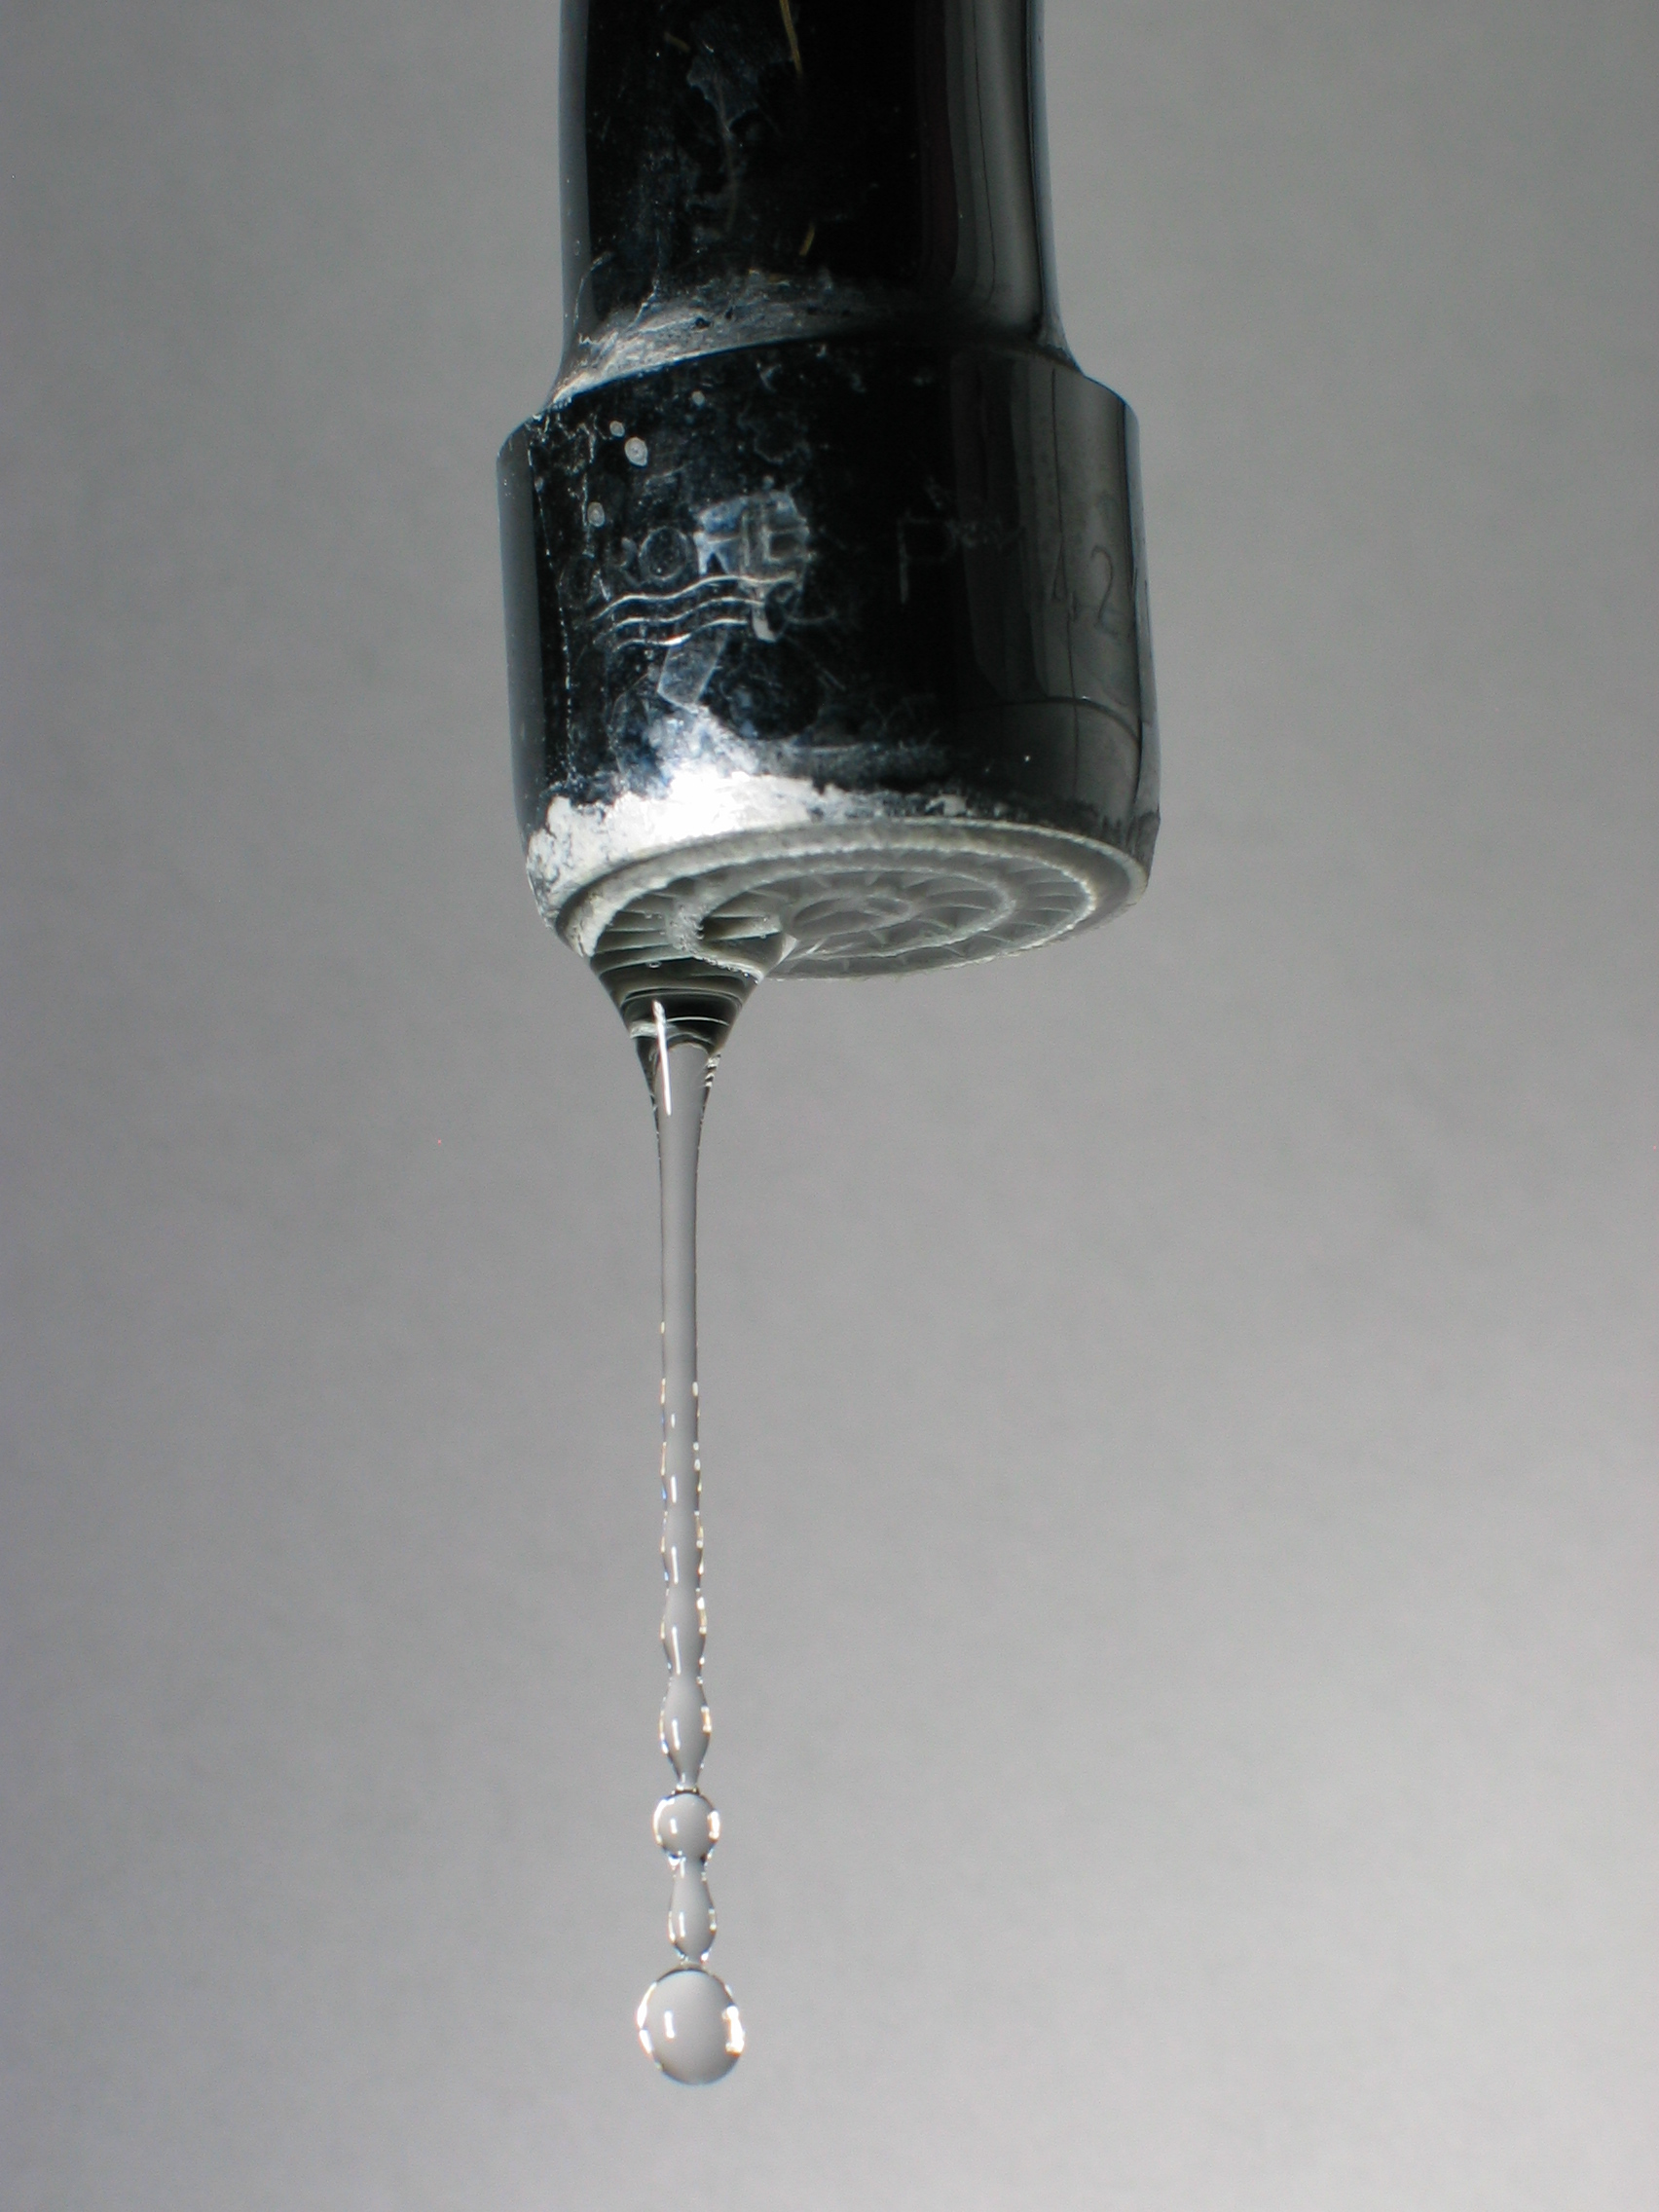
\includegraphics[scale=0.16]{png/Dripping_faucet_2.jpg}
  }\hfill
  \subcaptionbox{A breaking wave.\label{fig:intro:wave}}
  [0.65\textwidth]{
    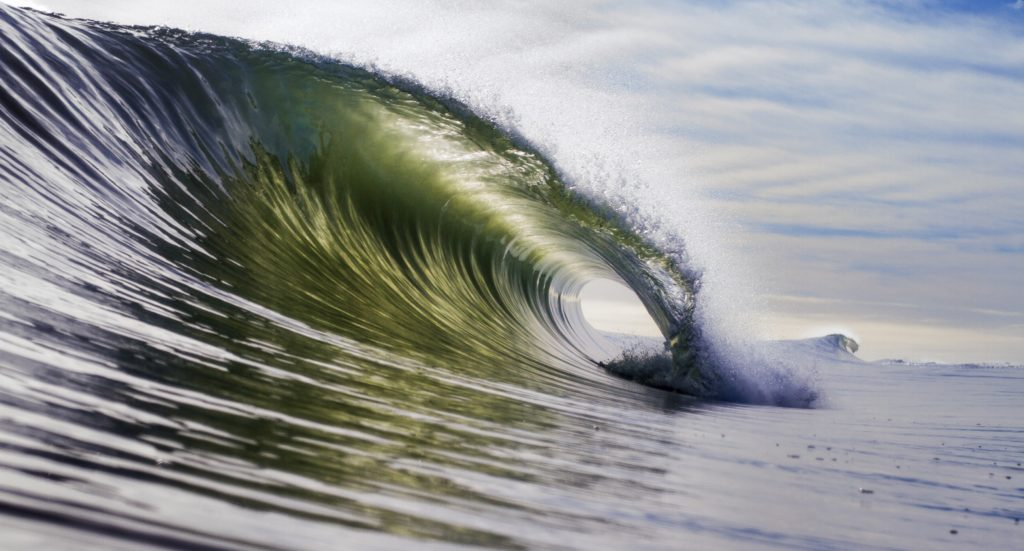
\includegraphics[scale=0.35]{png/shutterstock_509860879-breaking-wave-3720x2000-1024x551.jpg}
  }
  \caption{Examples of two-phase flow on different scales.}
\end{figure}
\lipsum[1-3]
  
  \partabstract{\itshape \lipsum[1]}
  \part{This is what the first part is about}\label{partone}
  % !TEX root = ./thesis.tex
\chapter{A chapter}\label{ch:int}

\begin{abstract}
  \lipsum[3-4]
\end{abstract}

% !TEX root = ./thesis.tex
\section{Introduction}
\lipsum[5]

\subsection{Specifics}
The following has a very difficult proof~\citep*{lagree2011granular_custom}, which can be found in~\cref{sec:app:exact_dr}.
\begin{restatable}[Very important theorem]{theorem}{thmimportant}\label{lem:int:centroid:unsplit_as_remap}
  For real numbers $x, y, z \in \mathbb{R}$ it holds that
  \begin{eqnarray}
    \abs{x - z} \le \abs{x - y} + \abs{y - z}.
  \end{eqnarray}
  % NOTE: autonum fails with thm-restate if the thm contains an equation, so instead we must use eqnarray and refer to it using \caref
\end{restatable}


\begin{corollary}[Obvious consequence]
  \begin{equation}
    \abs{1 -3} \le \abs{1 - 2} + \abs{2 - 3}.
  \end{equation}  
\end{corollary}
\begin{proof}
  Let $x = 1, y = 2$ and $z = 3$ in~\cref{lem:int:centroid:unsplit_as_remap}.
\end{proof}

\subsection{Volume of fluid method}
\begin{figure}
  \centering
  \import{inkscape/}{mass_transport.pdf_tex}
  \caption{\lipsum[6]}
  \label{fig:interface:mass_transport}
\end{figure}
The \gls{vof} method aims at tracking the volume of fluid per control volume, or equivalently the volume fraction in time.
Conservation of the total liquid (or equivalently gas) volume amounts to conservation of mass for incompressible fluids, as are considered here, and therefore the \gls{vof} method is a popular choice when mass conservation is of interest.
See also~\citet{Basilisk,IMO2020}.

If I want the acronym to be written in full, I use \glsentrylong{vof}, and if I want it to be written short: \glsentryshort{vof}, and both: \glsentryfull{vof}.
To have a clickable full reference we can use \glsfirst{vof}.


% \input{int_...}
% \input{int_...}
% \input{int_...}

\namedsubappendices
\begin{subappendices}
  \crefalias{section}{appendix}
  \section{Super hard proofs}\label{sec:app:exact_dr}

\thmimportant*
\begin{proof}
  \begin{table}
    \centering
    \begin{tabular}{cccccc}
      \toprule
      \multicolumn{3}{c}{Definition of $\pathlinetype{j}$} & \multicolumn{3}{c}{} \\
      \cmidrule{1-3}
       & & \multicolumn{4}{c}{$\+x_0 \in$} \\
      \cmidrule{3-6}
      $j$ & $\pindex^{\abs{\cdot}}_{\partial c}(\+x_0)$ & $c$ & $\drOne^+_c$ & $\drOne^-_c$ & $\mathcal{P}_c$\\ \midrule
      1 & 0 & N & N & N & N \\
      2 & 0 & Y & N & N & Y \\
      3 & 1 & N & Y & N & Y \\
      4 & 1 & Y & N & Y & N \\
      5 & 2 & N & Y & Y & N \\
      6 & 2 & Y & Y & Y & Y \\
      \bottomrule
    \end{tabular}
    \caption{Nice table}
  \end{table}
  The proof is left as an exercise for the reader.
\end{proof}

\end{subappendices}
  \cleardoublepage

  \addtocontents{toc}{\protect\newpage} % force new page in ToC for new part
  \partabstract{\itshape \lipsum[2]}
  \part{The second part is even more interesting}\label{parttwo}
  % !TEX root = ./thesis.tex
\def\thetitle{Transport of mass and momentum}
\chapter[\thetitle]{\thetitle\footnote{Based on a paper.}}\label{ch:twofluid1}
\chaptermark{\thetitle}

\begin{abstract}
  \lipsum[10]
\end{abstract}

\section{Introduction}\label{sec:pt1:introduction}
\lipsum[2]
\Cref{fig:intro:lgpi:1fluid_fine} is nice.

\begin{figure}
  \centering

  \subcaptionbox{Fine mesh using the \onefluid formulation.\label{fig:intro:lgpi:1fluid_fine}}
  [\threefigwidth]{
    \def\svgwidth{\threefigwidth}
    \import{inkscape/}{intro_lgpi_left.pdf_tex}
  }
  \hfill
  \subcaptionbox{Coarse mesh using the \onefluid formulation.\label{fig:intro:lgpi:1fluid_coarse}}
  [\threefigwidth]{
    \def\svgwidth{\threefigwidth}
    \import{inkscape/}{intro_lgpi_mid.pdf_tex}
  }
  \hfill
  \subcaptionbox{Coarse mesh using our proposed \twofluid formulation.\label{fig:intro:lgpi:2fluid_coarse}}
  [\threefigwidth]{
    \def\svgwidth{\threefigwidth}
    \import{inkscape/}{intro_lgpi_right.pdf_tex}
  }
  \caption{\lipsum[7]}
  \label{fig:intro:lgpi}
\end{figure} 
\section{Results}
Is there a \gls{rt} instability?

\begin{figure}
  \centering 
  \tikzsetnextfilename{lgpi_study_acceleration_legend}
  \inputtikz{lgpi_study_acceleration_legend}

  \captionbox{The interface profile several time instances.
  The arrows indicate the interface normal, with magnitude proportional to the interface normal velocity $u_\eta$.
  The solid marker indicates the left-most position of the lower part of the wave tip, and is used in~\cref{fig:results:wave3d:accel_normalvelo} to determine the wave tip acceleration.\label{fig:results:wave3d:accel_wavewithvelo}}
  [\twofigwidth]{
    \def\tikzWidth{\textwidth*0.35}
    \def\tikzHeight{\textwidth*0.35}
    \inputtikz{lgpi_study_tip_acceleration_wavewithvelo_custom}
  }\hfill
  \captionbox{The interface normal velocity as function of time, at the wave tip position as indicated by the markers in~\cref{fig:results:wave3d:accel_wavewithvelo}.
  The dashed line shows a linear least-squares fit with slope given by $\ddot{x}_\mtext{Tip} \approx -89\sivelocity$$^2$, which we subsequently use as the wave tip acceleration resulting in $\lambda_\mtext{\gls{rt}} \approx 9.8$mm.\label{fig:results:wave3d:accel_normalvelo}}
  [\twofigwidth]{
    \def\tikzWidth{\textwidth*0.35}
    \def\tikzHeight{\textwidth*0.35}
    \inputtikz{lgpi_study_tip_acceleration_normalvelo_custom}
  }
\end{figure} 

% \namedsubappendices
% \begin{subappendices}
%   \crefalias{section}{appendix}
%   \section{More }\label{sec:pt1:app:dr_analysis}

% \end{subappendices}

  % !TEX root = ./thesis.tex
\chapter{Conclusions and recommendations}\label{ch:conclusion}

\section*{Conclusions}
\lipsum[2]


\section*{Recommendations}
\lipsum[7]

  \backmatter
  {
    \renewcommand{\UrlFont}{\normalfont\small}
    \bibliography{custom_import}
  }

\end{document}
